%!TEX root = thesis.tex

\chapter{Visualisation Refinement}
\label{chap:visualisation-refinement}

Following the first user study (see Chapter~\ref{chap:user-study}), limitations of both the visualisations and the evaluation method were identified and corrective steps were taken. The steps taken to correct these limitations and the resulting refined visualisation are outlined in this chapter.

\begin{figure}
  \centering 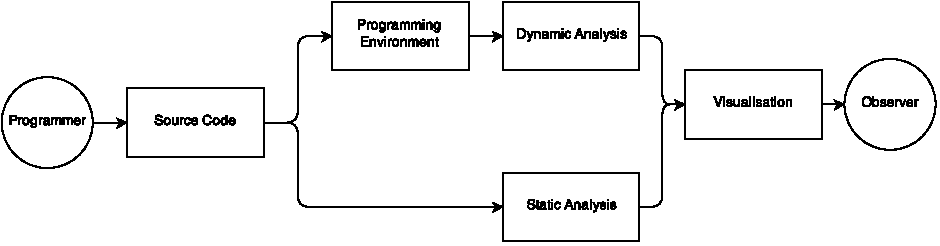
\includegraphics[width=\columnwidth]{../images/diagrams/knowledge-flow-refined.pdf}
  \caption{Knowledge flow from programmer to observer as directed by the visualisation technique employed.}
\label{fig:knowledge-flow-refined}
\end{figure}

\section{Rationale}

The initial user study (see Chapter~\ref{chap:user-study}) identified some improvement in enjoyment through the use of aesthetic visualisations. However, the study had conflicting results regarding understanding, with audiences reporting high levels of understanding attributed to the didactic visualisations when asked directly, but with lower overall understanding during the beginning stages of the live coding performance (see Section~\ref{section:user-study-understanding}). A new visualisation prototype was developed to bring together features identified as positively impacting enjoyment and understanding in one visualisation. This visualisation prototype built on a combination of the aesthetic and didactic visualisations evaluated in the previous study. The intention of this visualisation was to smooth the early transition into the more educational aspects of the visualisations through the aesthetic features identified.

Some technical limitations identified in the previous iteration of the visualisation prototype included incorrect timing and beat, no direct feedback from the programmer and limited links between the visuals and the source code. The goal of this iteration of the visualisation prototype was to rectify these issues while aligning the mental model of the audience with that of the programmer.

\section{Design}

As with the previous visualisation iteration, guidelines were identified, adapted and applied to the design process. Some of these design guidelines are outlined in Table~\ref{table:visualisation-refinement-guidelines} and are referred to in subsequent sections of the thesis.

{\renewcommand{\arraystretch}{2}
\begin{table}
  \centering
  \begin{tabular}{|p{6cm}|p{4cm}|p{3cm}|}
  \hline
  \textbf{Guideline} & \textbf{Reference} & \textbf{Identifier}\\
  \hline

Show relationships between entities using lines&\cite[p.~183]{Ware2013a}&\glab{guide:links}\\
\hline
``Consider using pictorial icons for pedagogical purposes in infographics.''&\cite[p.~320]{Ware2013a}&\glab{guide:icons}\\
\hline
``\ldots relate every beat\ldots~to the code responsible for that beat''&(see Section~\ref{section:improvements})&\glab{guide:code-responsible}\\
\hline
Respond to the programmer's typing&(see Section~\ref{section:liveness})&\glab{guide:typing}\\
\hline
Reduce visualisation distraction&(see Section~\ref{section:user-study-discussion})&\glab{guide:distraction}\\
\hline

  \hline
  \end{tabular}
  \caption{Additional guidelines for refinement decisions.}
  \label{table:visualisation-refinement-guidelines}
\end{table}
}

Three sources of data were to be combined and visualised: the state of the source code; the state of the running program; and the manipulation between the two by the live coder. To achieve this, three major components were required: an application manager; a code manager; and an editor plugin (see Figure~\ref{fig:visualisation-class-diagram}). The following sections detail the implementation of these components.

The refined model of knowledge flow from programmer to observer is shown in Figure~\ref{fig:knowledge-flow-refined}. As with the initial model of knowledge flow (see Figure~\ref{fig:knowledge-flow-initial}), dynamic analysis of the programming environment occurs. In this case however, the dynamic analysis is combined with static analysis of the source code before mapping to a visualisation.

\subsection{Visualisation Manager}

The visualisation manager handled all visual elements on the screen. The Polycode~\cite{Safrin2013} library was bound to the live coding environment allowing for more advanced two-dimensional graphical manipulations than the previous visualisation iteration through scene graph manipulation. Using this technique, the intention was to represent the state of the source code, the manipulation of the source code and the state of the active source code in the same visual environment.

\subsection{Interface Manager}
\label{sec:interface-manager}

To gather information regarding the actions of the programmer, a method of interfacing with the live coder's programming environment (text editor) was required. This was achieved using a text editor plugin sending programmer actions over an \ac{OSC} protocol. The interactions sent included cursor movement, all source code changes, file focus and source code evaluation. This protocol was implemented as a standard way of communicating between the text editor in use and the visualisations. Table~\ref{table:osc-protocol} describes the protocol.

Two text editor plugins implementing the protocol were developed including a plugin for EMACS~\cite{Stallman1981} and a plugin for Sublime Text~\cite{Skinner2013}.

\begin{table}
  \centering
  \begin{tabular}{|l|p{4.75cm}|p{4.75cm}|}
  \hline
  \textbf{OSC Address} & \textbf{Arguments} & \textbf{Description}\\
  \hline
	/interface/code & source\_code & Sent when the source code within the text editor changes.\\
	\hline
	/interface/evaluate & evaluated\_code & Sent when a block of source code within the text editor is evaluated (activated). \\
	\hline
	/interface/error & error\_text & Sent when an error occurs within the text editor or the evaluation of source code fails.\\
	\hline
	/interface/focus & file\_name & Sent when the file currently being edited changes.\\
	\hline
	/interface/cursor & cursor\_position \newline screen\_minimum\_position \newline screen\_maximum\_position \newline cursor\_position\_x \newline cursor\_position\_y & Sent when the text editor cursor selection changes. \\
  \hline
  \end{tabular}
  \caption{The OSC protocol developed for standardised interaction between text editors and the visualisation.}
  \label{table:osc-protocol}
\end{table}

\subsection{Code Manager}

Both static analysis of source code and dynamic analysis (see~\cite{Eisenbarth2003} and~\cite{Jerding1997}) of the program were combined into this iteration of the visualisation prototype in order to provide the audience with a link between the \acf{SoW} (the current active program) and the \acf{SoC} (the edits made to the source code not yet activated)~\cite{Swift2013}.

Static analysis of the source code involved parsing the source code written by the programmer and analysing any changes made, mapping these changes to historic source code states. The source code written by the programmer was sent from an editor plugin (see~\ref{sec:interface-manager}) to the Extempore visualisation program and stored as the current \ac{SoC}. Mappings to previous states were then made for each function within the source code.

Dynamic analysis of the running program involved providing mechanisms for the programmer to send running state information to be stored as the \ac{SoW}. A callback hook was provided to be used when creating an instrument during performance. This hook would provide data on the names of the instruments and the state of the callbacks, and would allow links to be determined between the \ac{SoC} and the \ac{SoW}.

\subsection{Mappings}

\begin{figure}
\centering
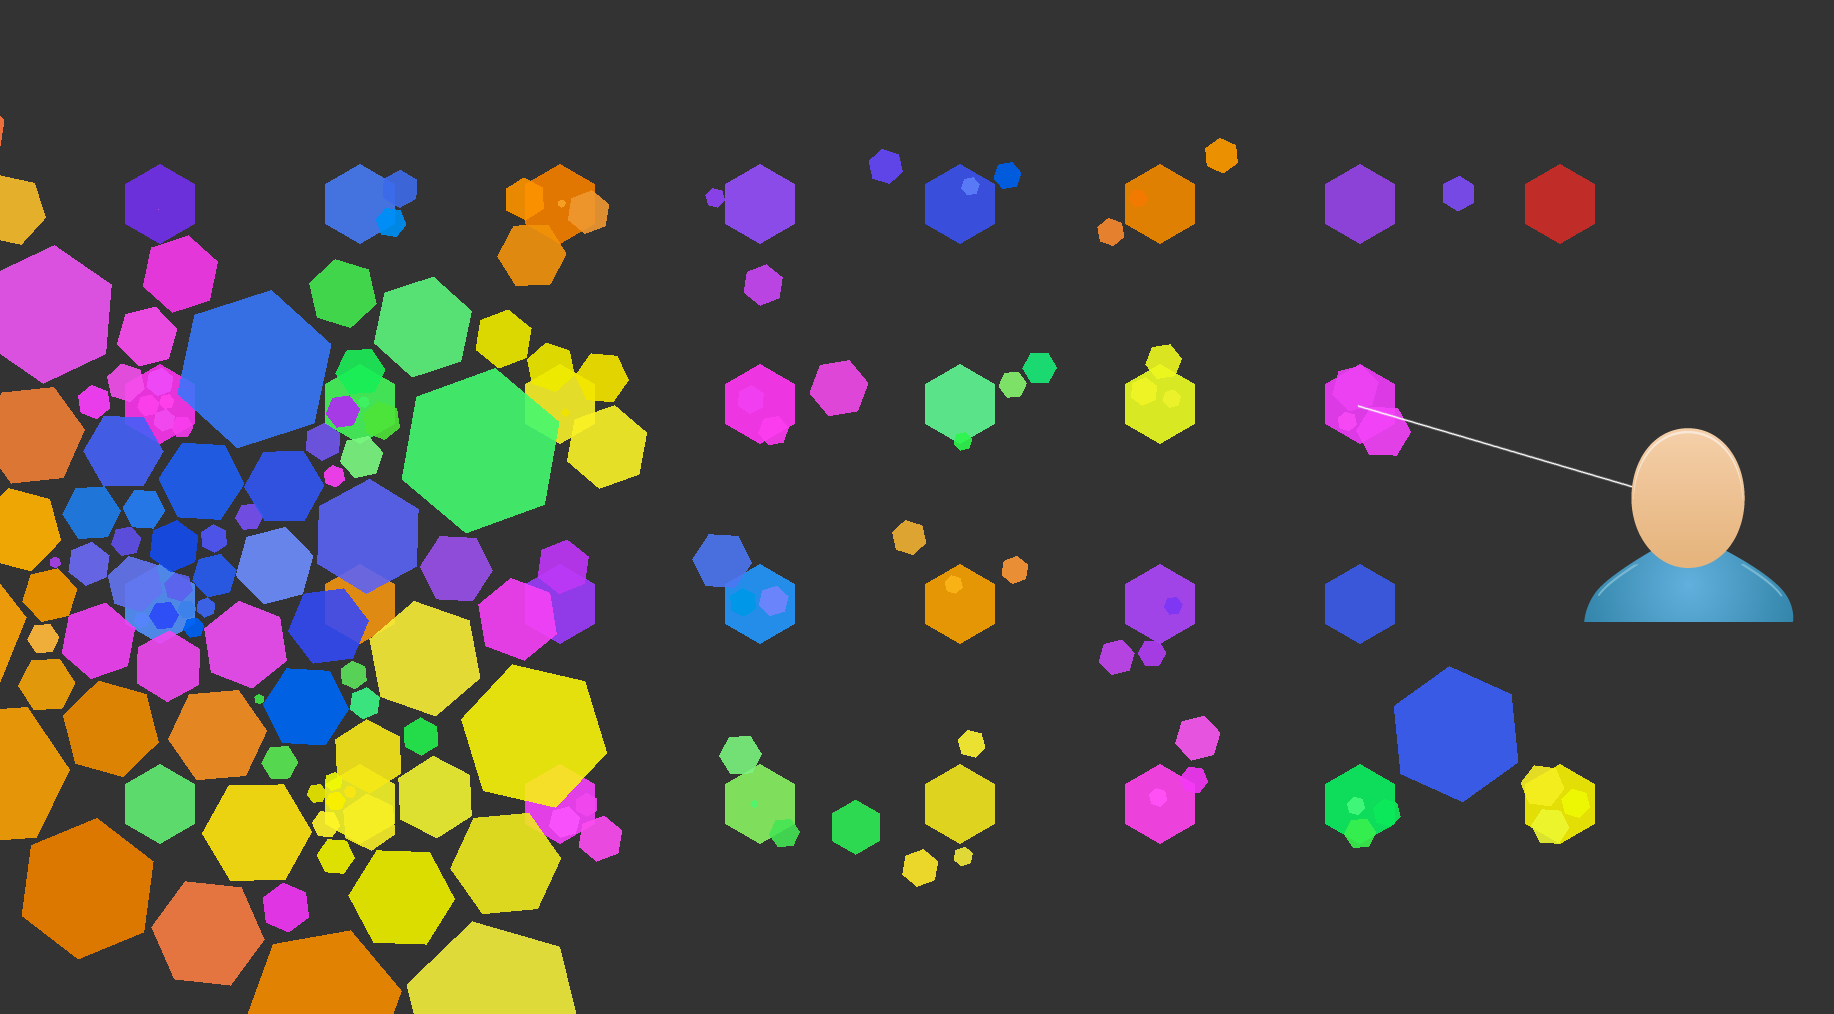
\includegraphics[width=\textwidth]{../images/final-visualisations/final-code-visualisation.png}
\caption{An example of the visualisation developed following the refinement process.}
\label{fig:final-visualisation}
\end{figure}

A number of specific mappings were assigned to the visualisation. These visual mappings related directly to actions taken by the programmer, behaviour of the running program and representation of the source code. 

Function count was mapped to the number of large visual elements on screen. When adding a new function, a new element was introduced. This mapping was intended to allow the audience to associate the simplified geometric shape to the source code and allow the audience to separate functions visually.

\begin{figure}
  \centering 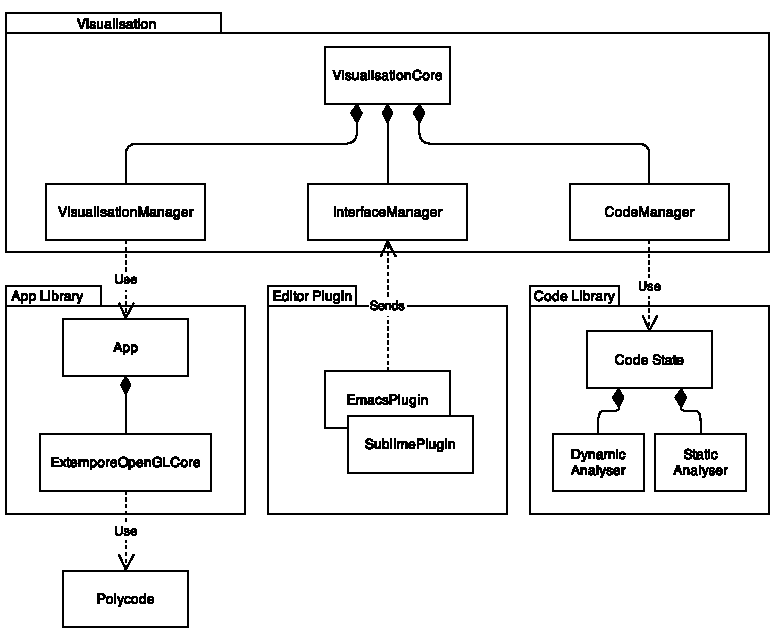
\includegraphics[width=\columnwidth]{../images/diagrams/visualisation-class-diagram.pdf}
  \caption[The refined visualisation class diagram]{The refined visualisation class diagram. The three major components included the visualisation manager, the interface manager and the code manager. The visualisation manager handled the mapping from the state of the live coding program to the visual elements. The interface manager received details of the state of the text editor from a text editor plugin. Finally, the code manager collected data from both the running live coding program and the static source code retrieved from the text editor to combine into the current state of the live coding program.}
\label{fig:visualisation-class-diagram}
\end{figure}

Each large visual element represented the state of active and inactive functions. In live coding, the programmer triggers functions to change between active and inactive states. The mapping represented this through the use of washed out grey and white shades while inactive, and vibrant, bright colours while active. In addition, the active functions were animated, with moving visual elements.

Function size and shape were represented visually through the use of ``attractors'' with each line of code mapped to one of the visual elements. Visual elements would grow and shrink according to the length of the line of source code directly mapping the typing actions of the programmer to visual elements.

To ensure the relationship between the actions of the programmer, the changes to the source code and the changes to the music were easily identified, an icon representing the programmer was displayed closest to the function being edited. This mapping intended to provide the audience with a better overview of the movements of the programmer among the functions than would otherwise be visible through the cursor alone.  

\section{Development}

A similar development approach to the previous iteration of the visualisation prototype was taken. This process involved collaborating with a live coding artist to further develop visualisations appropriate for the live coding context.

A strategy for combining static source code and the dynamic program structures was developed. This required storing the state of each function within the program comprised of the function change history, active state, current state and editing metadata. The function change history was extracted from source code sent from the text editor to the interface manager to be analysed.

Analysis of the source code involved parsing the source code and extracting functions and function names. It was determined early within the development process that full parsing of the syntax would not be necessary for informative visualisations. Instead, a heuristic line-by-line approach was implemented, separating functions in the source based on a set of simple rules. This approach allowed for managing syntax errors and incomplete syntax common while \textit{writing} a program. 

Development took an iterative approach, testing components thoroughly. Testing strategies employed included unit testing, integration testing and system testing. Low level unit tests were written for the three components of the visualisation system: the interface manager, the code manager and the visualisation manager. Integration testing was considered essential due to the large numbers of interacting components and was conducted throughout the development process. Finally, system testing (and to some extent, user testing) was conducted with the live coder to ensure correct functionality within the system as a whole.

\section{Summary}

In summary, this visualisation technique attempted to bring together effective features identified within the aesthetic and didactic visualisations of the previous iteration (see Chapter~\ref{chap:visualisation-design}). The prototype developed included three major components, consisting of the visualisation manager, the interface manager and the code manager. Technical limitations with the first iteration of the visualisation prototype were addressed and the state of the running program and the manipulation of the source code were mapped to visual elements. The effectiveness of aligning the mental models of the audience and the live coder was to be evaluated in a follow-up user study (see Chapter~\ref{chap:follow-up-user-study}).


